\section{D meson selection}
The \Dstar meson and their anti-particles was reconstructed in the central rapidity region by exploiting their charged hadronic decay channels: \Dstar $\rightarrow$ \Dzero$\pi^{+}$ (with B.R. = 67.7 $\pm$ 0.5$\%$), while the \Dzero meson decay into $K^-$ and $\pi^{+}$ with branching ratio (3.93$\pm$0.04)\%. The \Dstar decay proceeds via strong interaction, thus making impossible the secondary vertex reconstruction. The analysis exploits topological selections on the \Dzero,  together with the sharp peak in the difference between the invariant mass of the three final state hadrons and that of the two \Dzero decay prongs. Since the mass difference $\Delta m = m_{\rm D^{\ast +}} - m_{\rm D^0} \approx 145.4$ MeV/$c$ is only slightly larger than the charged pion mass. For low \pt \Dstar mesons the produced pion has typically low momentum and is referred to here as a soft pion.


%In this case the selection is applied to the decay topology of the daughter \Dzero. The selection of \Dzero candidates is based on the reconstruction of the displaced secondary vertex topologies, with a typical separation of $\sim$ 100$\mu$m from the interaction point. The \Dstar meson raw yields are extracted from the invariant mass distributions obtained from the analysis of fully reconstructed decay topologies displaced with respect to the primary vertex.

\subsection{Single track selections}
\label{sec:single_track}

The \Dstar candidates were formed by combining \Dzero candidates with soft pion $\pi^{+}$ tracks having $|\eta| <$ 0.8 and \pt $>$ 0.3 GeV/$c$, also satisfying the kITSrefit and kTPCrefit conditions. Moreover, for all the tracks, a minimum number of 70 crossed rows in the TPC together with a crossed rows over findable clusters ratio of 0.8 was required, and $\chi^2$/$ndf <$ 2 in the TPC. A cut on the transverse impact parameter $d_0$ was applied for tracks with \pt $<$ 2 GeV/$c$, requiring $d_0 >$ 50 $\mu$m. These selections were meant to limit the CPU time needed to perform the track combinatorics when creating the AODs with the D meson candidates. Furthermore, the \Dstar soft pions were selected requiring at least one associated hit in either of the two SPD layers.
% at least 70 out of 159 crossed TPC pad rows
% SetMinNCrossedRowsTPC(70)
% SetMinRatioCrossedRowsOverFindableClustersTPC(0.8)
% Moreover, for all the tracks, a minimum number of 70 crossed rows in the TPC together with a crossed rows over findable clusters ratio of 0.8 was required. 


  
  
%Secondary vertices of \Dzero and \Dplus meson candidates were constructed using tracks having $|\eta| <$ 0.8, \pt $>$ 0.5 GeV/$c$ and satisfying the kITSrefit and kTPCrefit conditions. Moreover, for all the tracks, a minimum number of 70 crossed rows in the TPC together with a crossed rows over findable clusters ratio of 0.8 was required. A cut on the transverse impact parameter $d_0$ was applied for tracks with \pt $<$ 2 GeV/$c$, requiring $d_0 >$ 50 $\mu$m. These selections were meant to limit the CPU time needed to perform the track combinatorics when creating the AODs with the D meson candidates. Furthermore, all tracks, including the \Dstar soft pion, were selected requiring at least 70 (out of a maximum of 159) associated space points and $\chi^2$/$ndf <$ 2 in the TPC, and at least one associated hit in either of the two SPD layers.

\subsection{Topological and kinematic selections}
%The yield extraction was performed using a particle selection strategy that has high efficiency and high statistical significance for the \Dstar meson signal.
%The same topological variables as in previous \Dstar -meson analyses were used in this analysis.

The \Dstar signal extraction is based on topological selections of displaced secondary vertices from \Dzero -meson candidates. For a detailed explanation of the procedure refer to \cite{Adam:2015sza}. The topological and kinematic cuts used to select the \Dstar -meson signal in pp collisions at \s 13 TeV are reported in Table~\ref{tab:CutDstar} and ~\ref{tab:CutDstar2}.

%The same topological and kinematic variables used for the analyses with the 2015 \pbpb data sample are reported. In particular, we recall the introduction of a topological variable introduced in \cite{Bruna:2016mgn} :

% the normalized impact parameter (IP) resolution. It is defined as the difference between the expected impact parameter value $d^{exp}_{0,T,\phi} \approx L_{xy} \cdot sin(\theta_{xy})$, where $L_{xy}$ is the decay length on $xy$ plane and $\theta_{xy}$ is the angle between the reconstructed D meson and the charged particle on $xy$ plane, and the reconstructed one $d^{reco}_{0,T,\phi}$. This difference is then normalized by the square root of their respective uncertainties summed in quadrature. A selection based on this variable can reduce the feed-down D-meson efficiency while keeping higher that of prompt D mesons. The projections of the variables in the $xy$ plane are instead justified by the improving of the impact parameter resolution with respect to $z$-direction. More details on this variable can be found in \cite{Bruna:2016mgn}.

%In addition, \Dsubs candidates were selected by requiring that one of the two pairs of oppositely-charged tracks had an invariant mass compatible with the PDG world average for the $\phi$ mass (1.019 GeV/$c^2$). 
%In order to further suppress the combinatorial background, the angles $\theta^{*}(\pi)$ and $\theta^{'}$(K) were exploited. 
%The first one is the angle between the pion in the KK$\pi$ rest frame and the KK$\pi$ flight line, which is defined by the positions of the primary and secondary vertices in the laboratory frame, and the second one is the angle between one of the two kaons and the pions in the KK rest frame.
%In order to further suppress the combinatorial background, the angle $\theta^{'}$(K) was exploited. This is the angle between one of the two kaons and the pions in the KK rest frame.


\begin{table}[h!]
  \begin{center}
    \caption{Selections used for the \Dstar -meson in the transverse momentum intervals 1$<$\pt$<$6.5 GeV/$c$.}  
    \label{tab:CutDstar}
    \resizebox{\linewidth}{!}{\begin{tabular}{|c|c|c|c|c|c|c|c|c|c|c|c|c|}
    \hline
      \pt (GeV/$c$) variable & [1-1.5] & [1.5-2] & [2-2.5] & [2.5-3] & [3-3.5] & [3.5-4] & [4-4.5] & [4.5-5] & [5-5.5] & [5.5-6] & [6-6.5] \\
      \hline
      \hline
      $\Delta M_{\rm D^0}$ (GeV)  & 0.021 & 0.032 & 0.035 & 0.035 & 0.038 & 0.038 & 0.038 & 0.042 & 0.042 & 0.045 & 0.049\\
      \hline
      DCA (cm) & 0.022 & 0.038 & 0.03 & 0.03 & 0.03 & 0.03 & 0.042 & 0.042 & 0.05 & 0.05 &  0.1 \\
      \hline
      $Cos(\theta^*)$ & 0.9 & 0.9 & 0.8 & 0.8 & 0.8 & 0.8 & 0.9 & 0.9 & 1.0 & 1.0 & 1.0  \\
      \hline
      \pt($K$) (GeV/$c$) & 0.4 &  0.4 & 0.9 & 0.9 & 0.9 & 1.0 & 1.0 & 1.0 & 1.0 & 1.0 & 1.0 \\
      \hline
      \pt($\pi$) (GeV/$c$) & 0.4 &  0.4 & 0.9 & 0.9 & 0.9 & 1.0 & 1.0 & 1.0 & 1.0 & 1.0 & 1.0 \\
      \hline
      $d_{0,K}$ (cm) & 0.1 & 0.1 & 0.1 & 0.1 & 0.1 & 0.1 & 0.1 & 0.1 & 0.1 & 0.1 & 0.1\\
	  \hline
	  $d_{0,\pi}$(cm)& 0.1 & 0.1 & 0.1 & 0.1 & 0.1 & 0.1 & 0.1 & 0.1 &0.1 &0.1 & 0.1 \\
	  \hline
	  $d_{0,K} \times d_{0,\pi}$ (10$^{-3}$) (cm$^2$) & -0.00025   &-0.00025  &  -0.00019& -0.00019 & -0.000144 &-0.000144  & -2.8 $\times 10^{-5}$ &-2.8 $\times 10^{-5}$  & 5.5 $\times 10^{-5}$ & 5.5 $\times 10^{-5}$ &0.0001 \\
	  \hline
	  $Cos(\theta_{point})$ & 0.8 & 0.8 & 0.9  & 0.9 & 0.89 & 0.89 & 0.81 & 0.81 & 0.79 & 0.79 & 0.7  \\
	  \hline
	  Inv. mass half width of \Dstar (GeV) & 0.3 & 0.3 & 0.3 & 0.3 & 0.3 & 0.3 & 0.3 & 0.3 & 0.3 & 0.3 & 0.3  \\
      \hline
      hal width of $\Delta M$ (GeV)  & 0.3 & 0.3 & 0.3 & 0.3 & 0.3 & 0.3 & 0.3 & 0.3 & 0.3 & 0.3 & 0.3\\
	  \hline
      \pt soft $\pi$ min (GeV/$c$) & 0.05 & 0.05 & 0.05 & 0.05 & 0.05 & 0.05 & 0.05 & 0.05 & 0.05 & 0.05 & 0.05 \\
      \hline
      \pt soft $\pi$ max (GeV/$c$) & 0.3 & 0.3 & 0.4 & 0.4 & 0.6 & 0.6 & 0.6 & 100 & 100 & 100 & 100 \\
      \hline
	  $\theta$ & 1.0 & 1.0 & 1.0 & 1.0 & 1.0 & 1.0 & 1.0 & 1.0 & 1.0 & 1.0 & 1.0\\
	  \hline
	  $|Cos(\theta_{point})XY|$ & 0.88 & 0.88 & -1. & -1. & -1. & -1. & -1. & -1. & -1. & -1. & -1. \\
	  \hline
	  $\rm NL_{XY}$ & 3. & 3. & 3. & 3. & 0 & 0 & 0 & 0 & 0 & 0 &  0 \\
	  \hline
    \end{tabular}
    }
  \end{center}
\end{table}



\begin{table}[h!]
  \begin{center}
    \caption{Selections used for the \Dstar -meson in the transverse momentum intervals 6.5$<$\pt$<$50 GeV/$c$.}  
    \label{tab:CutDstar2}
    \resizebox{\linewidth}{!}{\begin{tabular}{|c|c|c|c|c|c|c|c|c|c|c|c|}
    \hline
      \pt (GeV/$c$) variable & [6.5-7] & [7-7.5] & [7.5-8] & [8-9] & [9-10] & [10-12] & [12-16] & [16-24] & [24-36] & [36-50]  \\
      \hline
      \hline
      $\Delta M_{\rm D^0}$ (GeV)  & 0.049 & 0.052 & 0.052 & 0.056 & 0.056 & 0.074 & 0.074 & 0.074 & 0.074 & 0.074 \\
      \hline
      DCA (cm) & 0.1 & 0.1 & 0.1 & 0.1 & 0.1 & 0.1 & 0.1 & 0.1 & 10 & 10  \\
      \hline
      $Cos(\theta^*)$ & 1.0 & 1.0 & 1.0 & 1.0 & 1.0 & 1.0 & 1.0 & 1.0 & 10 & 10   \\
      \hline
      \pt($K$) (GeV/$c$) & 1.0 &  0.6 & 0.6 & 0.6 & 0.6 & 0.6 & 0.6 & 0.5 & 0.2 & 0.2  \\
      \hline
      \pt($\pi$) (GeV/$c$) & 1.0 &  0.6 & 0.6 & 0.6 & 0.6 & 0.6 & 0.6 & 0.5 & 0.2 & 0.2  \\
      \hline
      $d_{0,K}$ (cm) & 0.1 & 0.1 & 0.1 & 0.1 & 0.1 & 0.1 & 0.1 & 0.15 & 0.5 & 0.5 \\
	  \hline
	  $d_{0,\pi}$(cm)& 0.1 & 0.1 & 0.1 & 0.1 & 0.1 & 0.1 & 0.1 & 0.15 & 0.5 & 0.5 \\
	  \hline
	  $d_{0,K} \times d_{0,\pi}$ (10$^{-3}$) (cm$^2$) & 0.0001  & 0.0001 & 0.00019 & 0.0001 & 0.0001 & 0.001  & 0.001 & 1. & 1. & 1.  \\
	  \hline
	  $Cos(\theta_{point})$ & 0.7 & 0.7 & 0.7 & 0.7 & 0.7 & 0.7 & 0.7 & 0.2 & 0.2 & 0.2   \\
	  \hline
	  Inv. mass half width of \Dstar (GeV) & 0.3 & 0.3 & 0.3 & 0.3 & 0.3 & 0.3 & 0.3 & 0.3 & 0.3 & 0.3  \\
      \hline
      hal width of $\Delta M$ (GeV)  & 0.3 & 0.3 & 0.3 & 0.3 & 0.3 & 0.3 & 0.3 & 0.3 & 0.3 & 0.3 \\
	  \hline
      \pt soft $\pi$ min (GeV/$c$) & 0.05 & 0.05 & 0.05 & 0.05 & 0.05 & 0.05 & 0.05 & 0.05 & 0.05 & 0.05  \\
      \hline
      \pt soft $\pi$ max (GeV/$c$) & 100 & 100 & 100 & 100 & 100 & 100 & 100 & 100 & 100 & 100  \\
      \hline
	  $\theta$ & 1.0 & 1.0 & 1.0 & 1.0 & 1.0 & 1.0 & 1.0 & 1.0 & 1.0 & 1.0 \\
	  \hline
	  $|Cos(\theta_{point})XY|$ & -1. & -1. & -1. & -1. & -1. & -1. & -1. & -1. & -1. & -1. \\
	  \hline
	  $\rm NL_{XY}$ & 0 & 0 & 0 & 0 & 0 & 0 & 0 & 0 & 0 & 0  \\
	  \hline
    \end{tabular}
    }
  \end{center}
\end{table}


\subsection{Particle identification}
\label{sec:pid_sel}
The identification of the charged kaons and pions in the TPC and TOF detectors provide an additional information for the background rejection in the low momentum region. In order to assign K and/or $\pi$ masses to the decay tracks, cuts are applied to the difference in the expected and measured signals, which are the specific energy deposited (d$E$/d$x$) in the TPC and the time-of-flight for the TOF. A 3$\sigma$ compatibility was required to \Dstar candidate's daughters. When tracks were without TOF signal, only the TPC particle identification was used. Tracks with contradicting particle identification were considered to be non-identified and retained for further analysis. 
%For the \Dsubs, cuts were applied to the difference between the measured signals and those expected for a pion or a kaon. For \pt $<$ 8 GeV/$c$, where the signal over background is small, a track was considered compatible with the kaon or pion hypothesis if both its d$E$/d$x$ and time-of-flight were within 3$\sigma$ from the expected values. Tracks without a TOF signal (mostly at low momentum) were identified using only the TPC information and requiring a 2$\sigma$ compatibility with the expected specific energy loss. Triplets of selected tracks were required to have two tracks compatible with the kaon hypothesis and one with the pion hypothesis. In addition, since the decay particle with opposite charge sign has to be a kaon, a triplet was rejected if the opposite-sign track was not compatible with the kaon hypothesis. This particle identification strategy, applied at low momentum, preserves about 85$\%$ of the \Dsubs signal.

\subsection{Signal extraction}
\label{sec:sign_extr}
%The \Dstar raw yields were extracted by performing a fit to the invariant mass distribution with a function composed of a Gaussian for the signal and an exponential to interpolate the background shape. In particular, for \Dzero the exponential is used for \pt $>$ 3 GeV/$c$, while a pol3 and pol2 where used for 1-2 GeV/$c$ and 2-3 GeV/$c$ bins, respectively. 

%In case of \Dplus, signals are fitted with Gaussian and background is fitted with Polynomial2 which describes the shape of the background reasonably well. 

The \Dstar raw yields were extracted by performing a fit to the mass difference $\Delta M$ = $M$(K$\pi\pi$) - $M$(K$\pi$) distributions and the term describing the background shape is an exponential convoluted with a power law according to the equation:
\begin{equation}
	f_{bkg} = a\sqrt{\Delta M - m_{\pi}}\cdot e^{b(\Delta M - m_{\pi})}
\end{equation}
where $m_{\pi}$ is the pion mass and $a$ and $b$ are free parameters.

The \Dstar $\Delta M$ invariant mass distribution is shown in Figure~\ref{fig:Dstar_InvMass}. For \pt 1-1.5 GeV/$c$, the Power function was used to described the background shape. Figures~\ref{fig:Dstar_compar} and~\ref{fig:Dstar_compar2} show that for the first \pt bin $1<p_{\rm T}<1.5$ GeV/$c$, the Power function was better to describe the background shape than the function mentioned above, Power Law$\times$Exponential function. The \Dstar signal was successfully extracted in the range $1<$\pt$<50$ GeV/$c$. The goodness of the mass fit against the Monte Carlo (MC) expectations was checked in terms of mass peak $\sigma$ and position.
The comparisons of the Gaussian width and mean of the \Dstar meson mass peaks in data and MC are reported in figure~\ref{fig:Dstar_Mean_width}.


% Dstar 0-10% InvMass plot
\begin{figure}[tb]
\begin{center}
 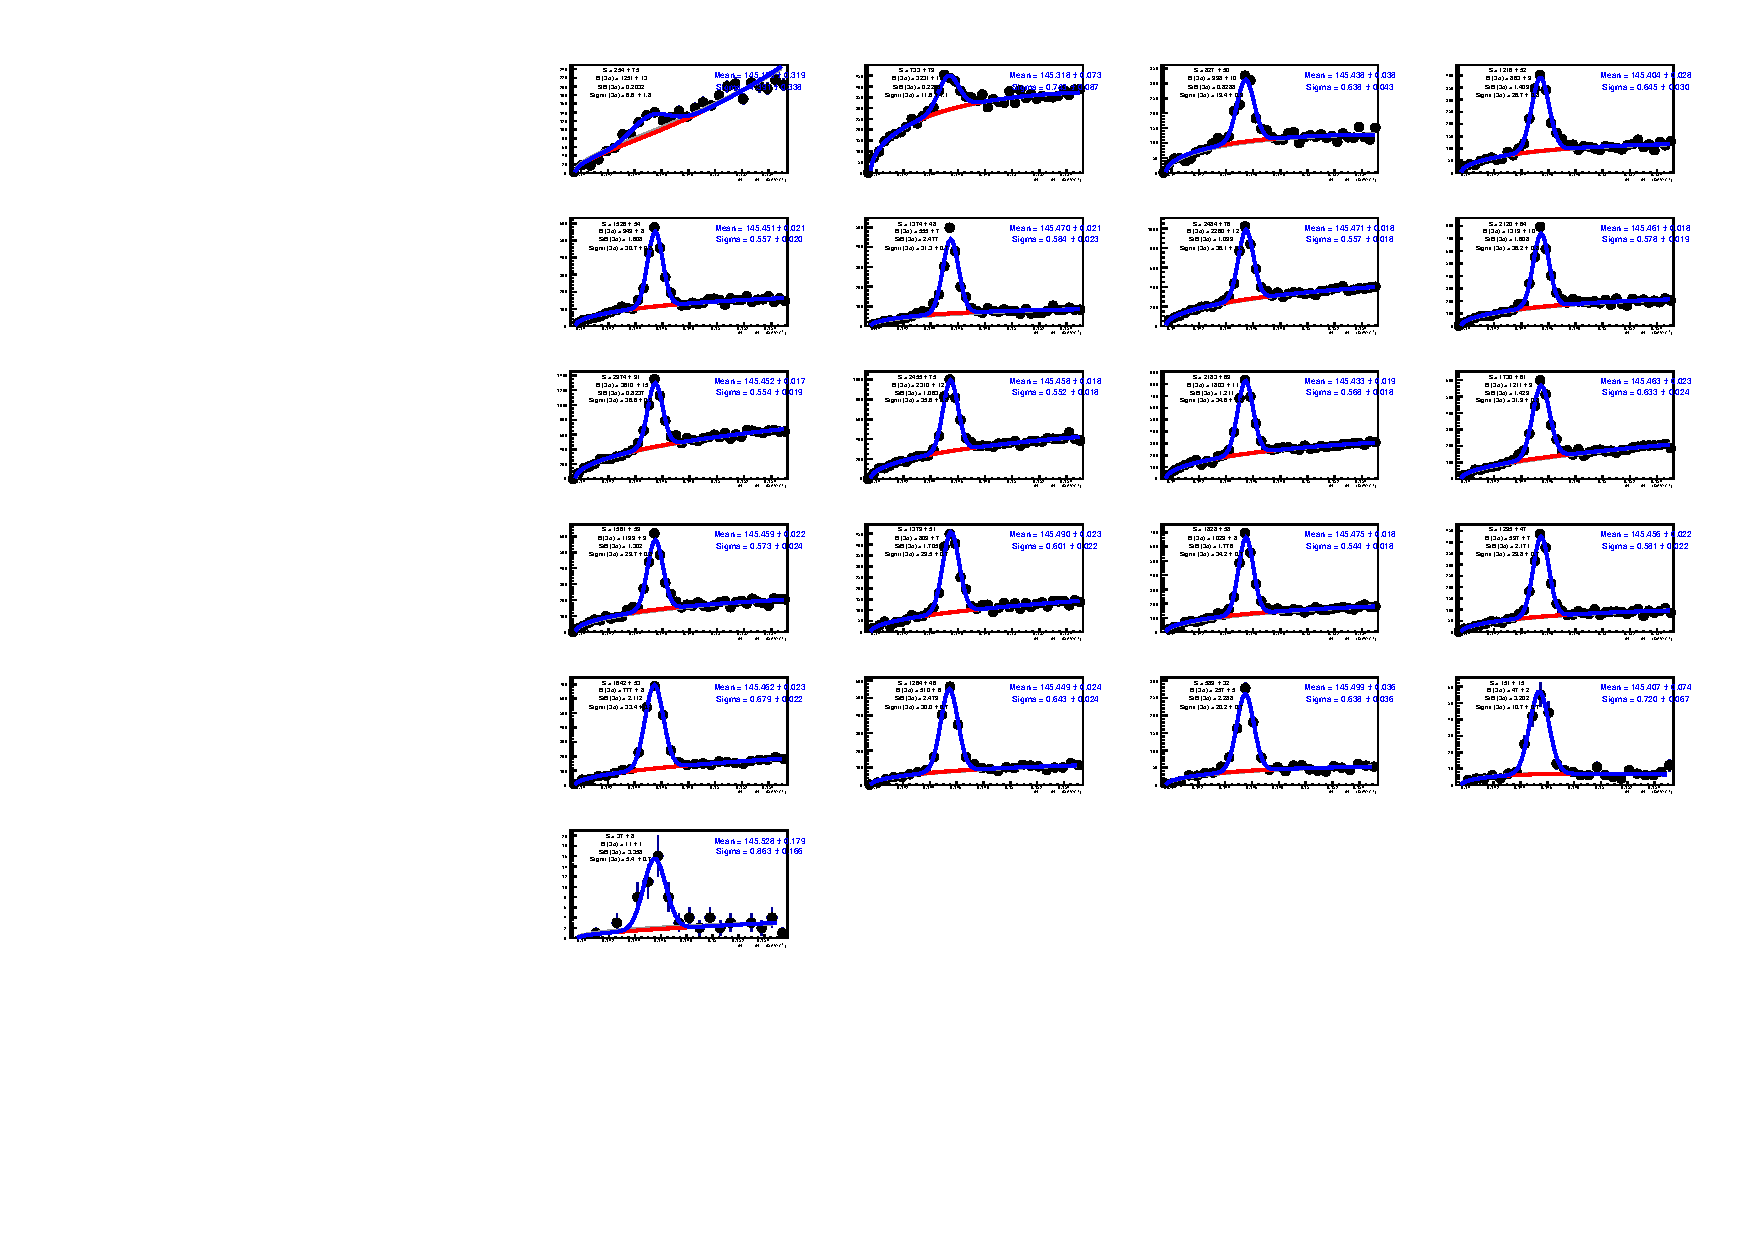
\includegraphics[width=1\textwidth]{figures/Dstar/pp13TeV/DstarInvMass_new.pdf}
\caption{Invariant mass distributions of  (\Dstar -- \Dzero) candidates and charge conjugates in the range 1$<$\pt$<$50 GeV/$c$.}
\label{fig:Dstar_InvMass}
\end{center}
\end{figure}


% Dstar Mean and width Data vs MC 0-10%


% Dstar Mean and width Data vs MC 30-50%
\begin{figure}[tb]
\begin{center}
 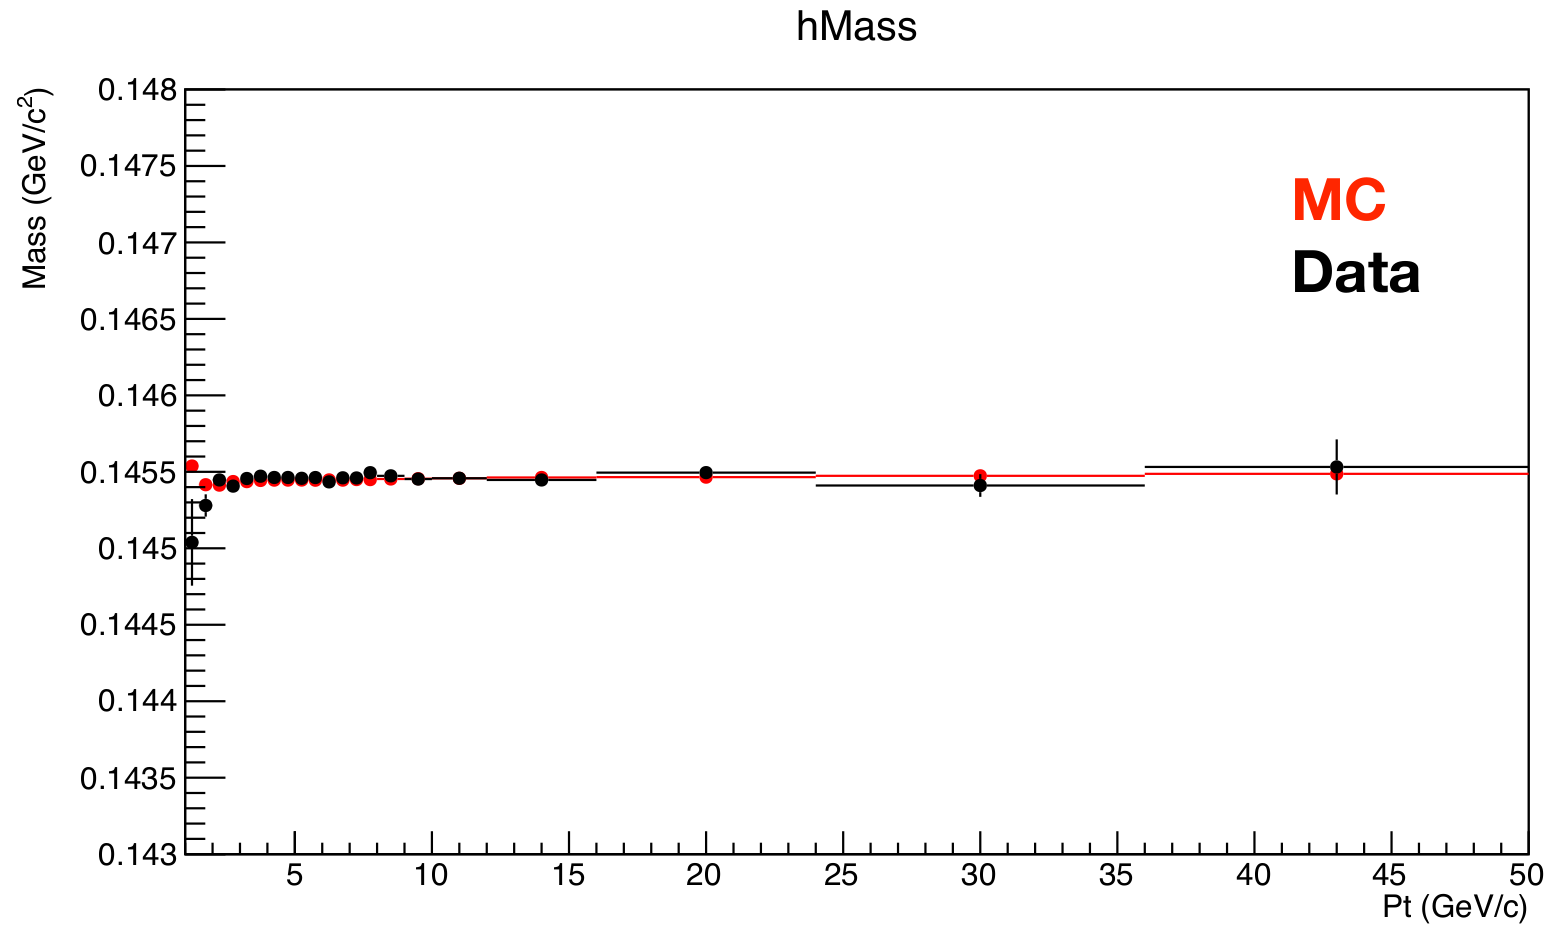
\includegraphics[width=0.65\textwidth]{figures/Dstar/pp13TeV/DstarMean-position.png}
 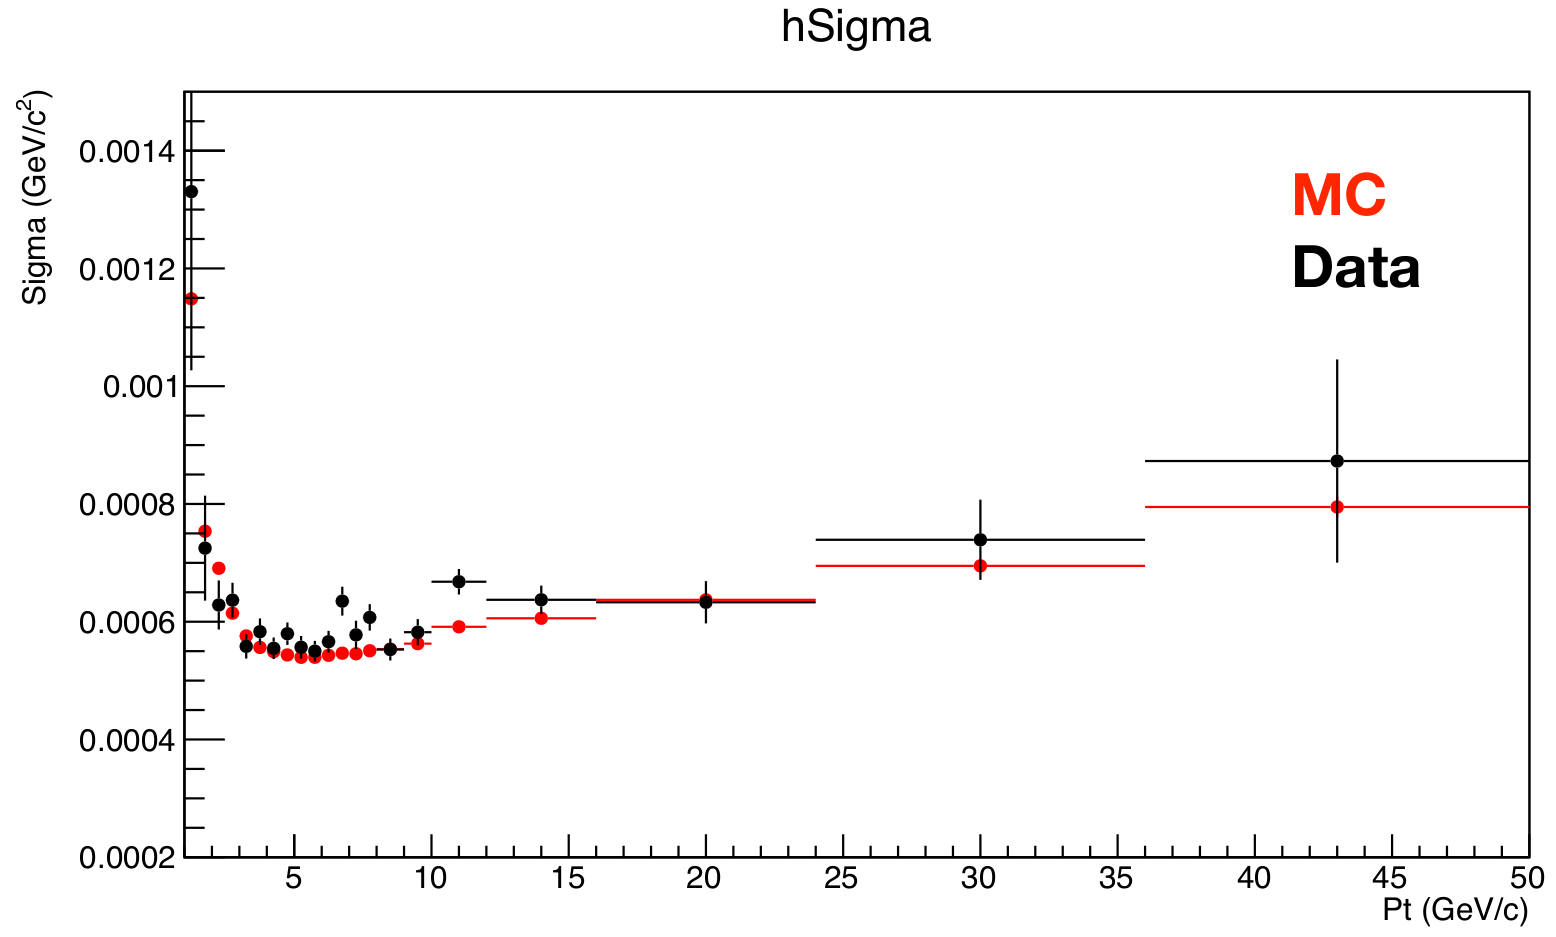
\includegraphics[width=0.65\textwidth]{figures/Dstar/pp13TeV/DstarWidth_sigma.png}
\caption{Comparison of Gaussian mean (top) and width (bottom) extracted from the invariant-mass fits of \Dstar
candidates (black) and the MC simulation (red).}
\label{fig:Dstar_Mean_width}
\end{center}
\end{figure}

% Dstar Mean and width Data vs MC 30-50%
\begin{figure}[tb]
\begin{center}
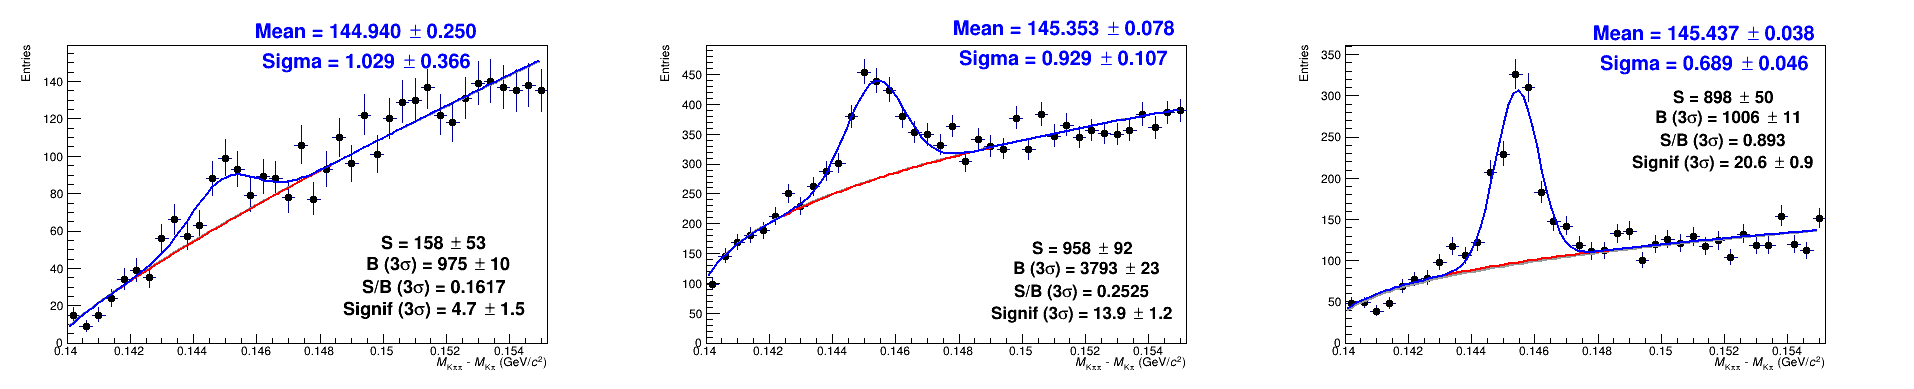
\includegraphics[width=1\textwidth]{figures/Dstar/pp13TeV/multi_trial/Figure_01.png} 
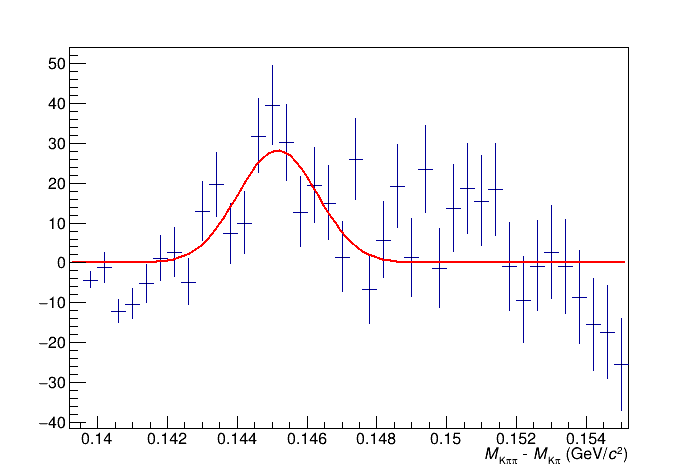
\includegraphics[width=0.32\textwidth]{figures/Dstar/pp13TeV/multi_trial/residual_plot_std_bkg_func_1-1dot5GeV.png} 
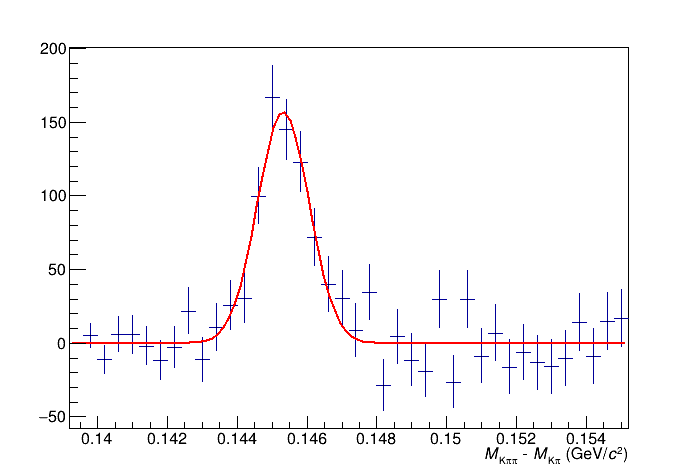
\includegraphics[width=0.32\textwidth]{figures/Dstar/pp13TeV/multi_trial/residual_plot_std_bkg_func_1dot5-2GeV.png}
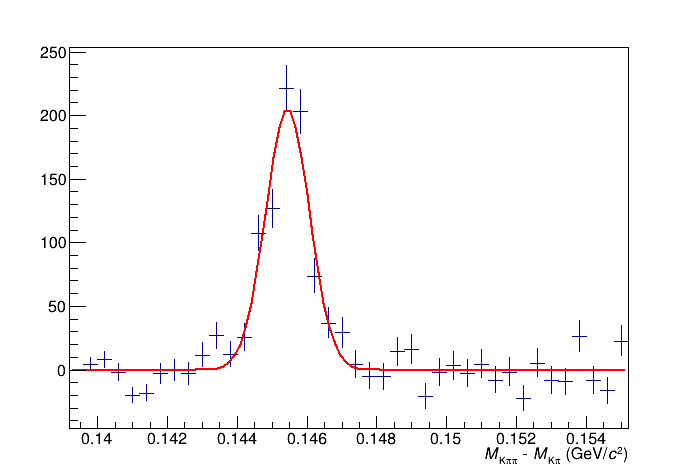
\includegraphics[width=0.32\textwidth]{figures/Dstar/pp13TeV/multi_trial/residual_plot_std_bkg_func_2-2dot5GeV.png} 
\caption{The \Dstar $\Delta M$ invariant mass distribution for \pt range 1-2.5 GeV/$c$ (top rows) with the Power Law$\times$Exponential function for describing the background shape and the residual plots (bottom rows).}
% The \Dstar $\Delta M$ invariant mass distribution for \pt range 1-2.5 GeV/$c$ (top rows) using the Power Law$\times$Exponential function and the residual plots (bottom rows).
\label{fig:Dstar_compar}
\end{center}
\end{figure}

\begin{figure}[tb]
\begin{center}
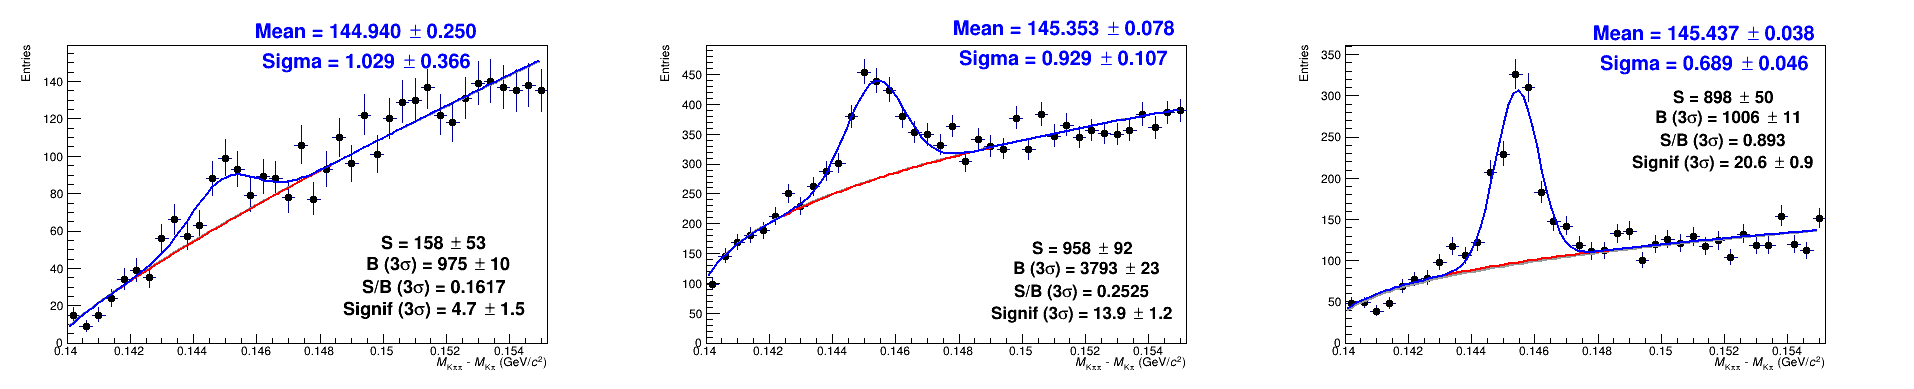
\includegraphics[width=1\textwidth]{figures/Dstar/pp13TeV/multi_trial/Figure_01.png}
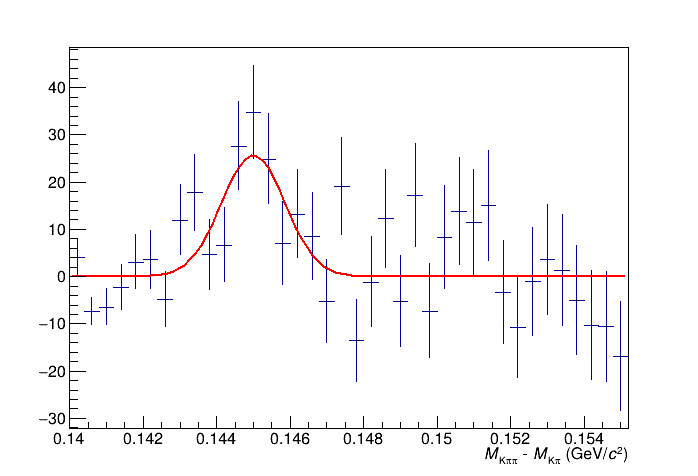
\includegraphics[width=0.32\textwidth]{figures/Dstar/pp13TeV/multi_trial/residual_plot_Pow_bkg_func_1-1dot5GeV.png} 
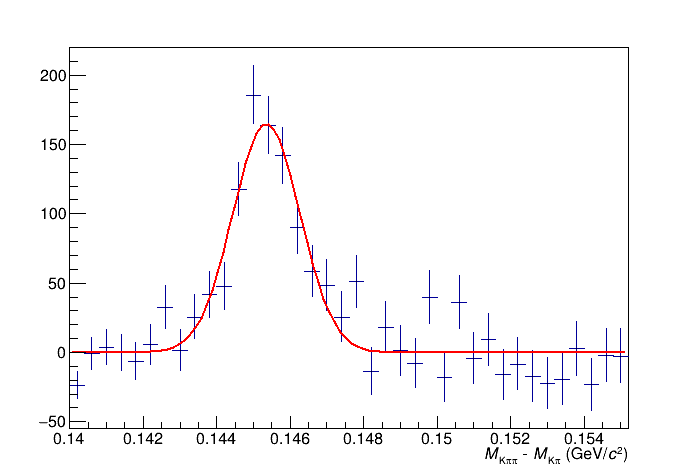
\includegraphics[width=0.32\textwidth]{figures/Dstar/pp13TeV/multi_trial/residual_plot_Pow_bkg_func_1dot5-2GeV.png}
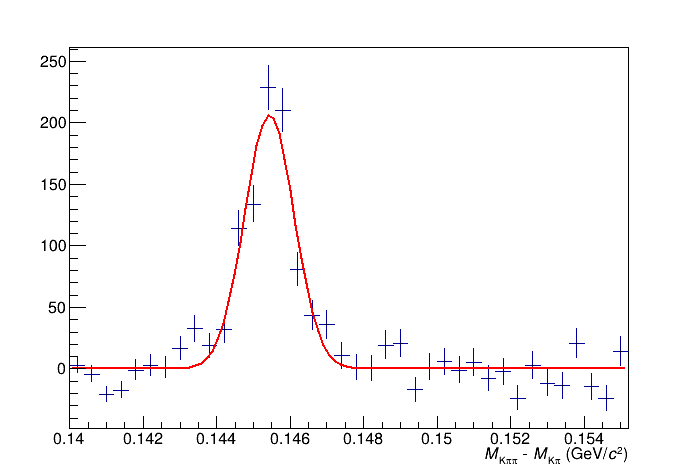
\includegraphics[width=0.32\textwidth]{figures/Dstar/pp13TeV/multi_trial/residual_plot_Pow_bkg_func_2-2dot5GeV.png} 
\caption{The \Dstar $\Delta M$ invariant mass distribution for \pt range 1-2.5 GeV/$c$ (top rows) with the Power Law function for describing the background shape and the residual plots (bottom rows).}
\label{fig:Dstar_compar2}
\end{center}
\end{figure}


% Dplus 0-10% Mean and Width
%\begin{figure}[tb]
%\begin{center}
% \includegraphics[width=1\textwidth]{figures/Dplus/010/meansigma_Comp_010_Pol2andExpo.pdf}
% \caption{Comparison of Gaussian mean (left) and width (right) extracted from the invariant-mass fits of \Dplus candidates in 0--10\% for the data and the MC simulation.}
%\label{fig:Dplus_Mean_width}
%\end{center}
%\end{figure}

% Dplus 30-50% Mean and Width
%\begin{figure}[tb]
%\begin{center}
% \includegraphics[width=1\textwidth]{figures/Dplus/3050/meansigma_Comp_3050_Pol2andExpo.pdf}
% \caption{Comparison of Gaussian mean (left) and width (right) extracted from the invariant-mass fits of \Dplus candidates in 30--50\% for the data and the MC simulation.}
%\label{fig:Dplus_Mean_width2}
%\end{center}
%\end{figure}




% Dstar 30-50%




%\begin{figure}[tb]
%\begin{center}
% \includegraphics[width=0.48\textwidth]{figures/Dsubs/010/Mean_Data_MC.pdf}
% \includegraphics[width=0.48\textwidth]{figures/Dsubs/010/Sigma_Data_MC.pdf}
%\caption{Comparison of Gaussian mean (left) and width (right) extracted from the invariant-mass fits of \Dsubs candidates in 0--10\% for the data and the MC simulation.}
%\label{fig:DsubsMCcomp_cent}
%\end{center}
%\end{figure}

%\begin{figure}[tb]
%	\begin{center}
%	 \includegraphics[width=0.48\textwidth]{figures/Dsubs/3050/CompMean.pdf}
%	 \includegraphics[width=0.48\textwidth]{figures/Dsubs/3050/CompWidth.pdf}
%	\caption{Comparison of Gaussian mean (left) and width (right) extracted from the invariant-mass fits of \Dsubs candidates in 30--50\% for the data and the MC simulation.}
%	\label{fig:DsubsMCcomp_semicent}
%	\end{center}
%	\end{figure}
